\documentclass[conference]{IEEEtran}
\IEEEoverridecommandlockouts
% The preceding line is only needed to identify funding in the first footnote. If that is unneeded, please comment it out.
\usepackage{cite}
\usepackage{amsmath,amssymb,amsfonts}
\usepackage{algorithmic}
\usepackage{graphicx}
\usepackage{textcomp}
\usepackage{xcolor}
\usepackage{hyperref}
\hypersetup{
    colorlinks=true,       % Makes the links colored (not boxed)
    linkcolor=blue,        % Color of internal links (sections, etc.)
    urlcolor=blue,         % Color of external links (URLs)
    citecolor=blue         % Color of citation links
}
\def\BibTeX{{\rm B\kern-.05em{\sc i\kern-.025em b}\kern-.08em
    T\kern-.1667em\lower.7ex\hbox{E}\kern-.125emX}}
\begin{document}

\title{Kyasanur Forest disease detection using LSTM-CNN, GRU, Transformer Networks\\
{\footnotesize \textsuperscript{}}

}

\author{\IEEEauthorblockN{Yetukuri Gargeya Sreenadh }
\IEEEauthorblockA{\textit{Dept. of Computing Technologies 
} \\
\textit{SRM Institute of Science and 
Technology}\\
Tamil Nadu, India  \\
gy0475@srmist.edu.in}
\and
\IEEEauthorblockN{Jaswanth Marni}
\IEEEauthorblockA{\textit{Dept. of Computing Technologies 
} \\
\textit{SRM Institute of Science and 
Technology}\\
Tamil Nadu, India  \\
jm2557@srmist.edu.in}
\and
\IEEEauthorblockN{Dr. Manjula Rajagopal}
\IEEEauthorblockA{\textit{Dept. of Computing Technologies 
} \\
\textit{SRM Institute of Science and 
Technology}\\
Tamil Nadu, India  \\
manjular1@srmist.edu.in}

}

\maketitle

\begin{abstract}
This project entitled "Kyasanur Forest Disease Prediction Using CNN-LSTM, GRU and Transformer Networks," is aimed at making predictions and early detection of Kyasanur forest disease (KFD), a tick-borne viral hemorrhagic fever that is endemic to South Asia. The project uses modern deep learning strategies and predictions based on a dataset of clinical signs and symptoms (e.g., fever, headache, joint pain), metadata from patients (e.g., GPS location, occupation), and blood-related symptoms (i.e., bloody nose, blood in stool). After preprocessing the dataset, which included missing data treatment, feature encoding, and normalisation, the final dataset was appropriate for model training.Three models performed the task; CNN-LSTM, GRU model and transformer networks. CNN-LSTM performs multiple convolutions to extract the spatial categorical feature and transfers the output to LSTM layers, which understands temporal sequences of the category values. The GRU model performs as a sequence with the added advantage of simpler sequential learning. The last model established a relationship between multi-dimensional feature and uses self-attention to make reliable and scalable predictions. The models were assessed using a set of performance metrics (accuracy, precision, recall, F1-score), and the transformer model performed better than both of the sequential models.This work demonstrates the emerging variable of AI that can enable advanced healthcare prediction for KFD, providing an efficient solution process for diagnosis in the healthcare field, as well as maintaining expectations for future advances pointing to new levels of real-time data, and expanding datasets for research on KFD. They will mark a great leap forward in the evolution of healthcare diagnostics.

\end{abstract}

\begin{IEEEkeywords}
Kyasanur Forest Disease (KFD) Early Detection; Deep Learning, Health Care Diagnostics; AI; Disease Detection; CNN-LSTM, GRU, Transformer Networks; Clinical Data; Pre-processing; Classifier Accuracy; Scalability; Public Health; and Real-time Data Integration.
\end{IEEEkeywords}

\section{Introduction}
Kyasanur Forest Disease (KFD) is a tick-borne viral hemorrhagic fever, which has recently developed into an important public health problem, particularly in endemic areas in South Asia. Human infections are possible via contact with infected ticks that are present in some tropical forests posing serious threats to human health. The clinical manifestation of KFD varies based on rate of progression, symptoms such as, fever, headache, joint pain, vomiting, bloody nose, blood in stool, internal bleeding, gastric bleeding and other serious hemorrhagic effects occur. These complications lead to the rational and timely diagnosis of KFD being the most important potential health impact, and ultimately health outcomes. Traditionally diagnostic rules for infectious disease have been truthful and false diagnoses however appropriate timing in assessing and analyzing patient health status have also been exactly delayed, have been costly, and/or have limited access to, in remote rural parts of the endemic KFD region. In addressing the evaluation and analysis aspect of serious health conditions of KFD, the project utilizes sources of accessible artificial intelligence, deep learning methods to produce predictive models of KFD. It includes clinical and demographic data systemically on the patients KFD profile, details of their symptoms, demographic identifiers differentiating diagnostic metadata and blood characteristics, such as GPS locations, occupation, and access to appropriate food and water sources. When having an opportunity to have scalable, efficient, scalable models, with automation such as storing, mining, analyzing and predicting, the anticipated clinical outcome in a potentially efficient diagnostic conception of using artificial kilobytes/milli-seconds approach for diagnosing KFD, could actually deliver on potential public health outcomes or improve baseline health systems in abandoning endemic situations in specific KFD setting areas. Then we will have the potential opportunity of using the diagnostic to prioritize patients for interventions.
\par\vspace{1em}
The study uses three contemporary cutting-edge deep learning models—CNN-LSTM, GRU, and Transformer Networks—to predict the occurrence of Kyasanur Forest Disease (KFD) based on clinical and demographic components of medical dataset. The (CNN-LSTM) model combines convolutional layers to extract spatial features while implementing (LSTM) layers to analyze temporal data, and making it the most appropriate model to process sequential patterns present in a medical dataset. Although the (GRU) model does not leverage convolutional or recurrent mechanisms, it has a simpler architecture that enhances sequence learning while minimizing the computational demands to a user with resource constraints. Similarly, (Transformer Networks) use self-attention mechanisms to provide better quality scalable predictions, because it captures long-term dependencies in historical data. The models are trained from a rigorously preprocessed dataset that contains clinical symptoms, demographics or other metadata on the patient, and quantitative indicators, such as blood. Preprocessing features include method for encoding features, normalizing features, and preparing features for missing values. The purpose of the study is to demonstrate the transformative powers of artificial intelligence in the domain of healthcare by depicting a scalable and efficient solution that leverages the research project’s larger pool of (KFD) cases as predictors for disease. The research suggests that integrating sophisticated technologies can be an effective means to improve public health in the developing world, offering hope for the ability to predict a disease within a population with little healthcare access. By identifying the research project as being founded on a technological intervention that recommends a proactive solution to combat pressing healthcare problems, the (KFD) research project clearly demonstrates that (AI) can address pressing healthcare challenges.
\section{Literature Survey}

The Transformer architecture introduced by Vaswani et al. (2017) represents a major breakthrough in deep learning targeted towards natural language processing tasks. Unlike traditional recurrent neural networks (RNNs), which process input data sequentially, Transformers make it possible to process input sequences as a whole with its self-attention mechanism. This feature also allows for a highly accelerated training process and large scale for big data. Self-attention layers in the Transformer architecture provide a means for the architecture to remember relevant parts of the data, simplifying the implementation of long-term dependencies between the input variables. As the flexibility and robustness of the Transformer increased, the use of Transformers increased from natural language processing applications to other application domains such as healthcare. Particularly, Transformers have been applied to disease prediction tasks and multi-dimensional datasets with complex interdependencies like a patient's clinical data and demographics. In the context of this project, using Transformer Networks is central in addressing the massive, heterogeneous inputs of our patients (symptoms), patient metadata and blood-related inputs as an example. Transformer networks possess powerful features in understanding complex relationships in structured data, to produce robust, scalable predictions especially for complex disease like Kyasanur Forest Disease (KFD). This work will be a focus for the development of the Transformer network based approach in this project, representing a technology-based opportunity for early disease prediction and prevention for public health.
\par\vspace{1em} 
Gupta et al. (2021) investigate hybrid CNN-RNN methods of malaria and dengue prediction including work with epidemiological factors, where CNN layers typically perform a sequence of spatial feature extractions and RNN layers capture temporal patterns of the disease ranging across the geographical, environmental, and temporally constructed features. The CNN layers applied were for structured epidemiological data, and the RNN layers were facilitating temporal modelling of outbreaks. They identified a very useful application of combining the time series nature with spatial representation information and produced better predictive accuracy through model improvements exploiting both types of prediction biases. In this project the hybrid CNN-LSTM model has similarities to Gupta et al. (2021). The clinical data is processed by the CNN layers then and the LSTM layers study the temporal aspects of the data (e.g., patient history, disease progression). Their work on exploiting the combined prediction aspects of using a CNN and RNN shows potential for fine-tuning model design and will inform how model architectures can be developed for disease prediction tasks. By implementing the hybrid model on KFD data, that consider both spatial (location specific outbreaks) and temporal (e.g., seasonality) patterns, we will optimize for prediction accuracy. This work can be leveraged as a starting point for implementing hybrid methods to health diagnostics.
\par\vspace{1em} 
Kumar et al., (2020) assessed the use of LSTM networks for predicting chronic conditions such as diabetes and hypertension, which make temporal predictions easy due to their sequential nature. They formulated their model from time-disaggregated patient data, clinical symptoms, crude reports, and laboratory results obtained over time. They demonstrated that their model consistently achieved disease prediction of a high degree of accuracy. This literature reference is relevant to our project, as it deals in temporal data, like the time-dependent data that displays later stages of symptoms and variable symptoms of KFD (KFD Detections). The strength of LSTMs is that they retain important long-term associations as the LSTMs model past data members completely, so nothing critical would be lost in coordination across LSTM layers, which will lead to more accurate predictions with the predictions occurring faster. Kumar et al., (2020) concluded that normalization and feature encoding were two important preprocessing steps that enhanced their model performance and meaningfulness (another part of the project methodology). They used an LSTM-based technique, and in our project, we will also design an LSTM, taking on a certain level of assumptions and relationships with KFD, and building upon its establishment for meaningful meaning for early prediction of the progression of disease (KFD Detections). Therefore, this reference will be absolutely beneficial in developing and validating heterogeneous architectures based on LSTM structures and for optimal and correct multi-layer LSTM model selections, as part of a hybrid model we developed for health-related applications; particularly as they relate to KFD Detections.
\par\vspace{1em}
The possibilities of Gated Recurrent Units (GRU) as a time-series method low-based predictions on healthcare were studied by Zhang et al. (2019) concentrating mainly on cardiovascular disease predictions. Now, the GRU is a more simplified version of recurrent neural networks (RNNs) but lesser computational-intensive than Long-Short-Term-Memory (LSTM) models. This makes the GRU advantageous in this study as the current project focuses on resource-poor scenarios where CRFs and LSTMs could be very demanding in computation. In their study, Zhang et al. revealed salient ways in utilizing gray uncertainty at clinical datasets using GRU models but at a significantly lower cost in computation power, which is also relevant for the current study focusing on resource-poor settings or KFD impact. Zhang et al. highlighted the importance of preprocessing steps such as transforming missing data values and normalizing data values to build more robust models. These preprocessing techniques are incorporated into this project to incorporate usable input into the GRU models. Zhang et al. offered evidence supporting the plausibility of GRUs and their ability to evaluate disease prediction tasks that require sequential data, for example, patient symptoms or timelines of disease progression. The project which is currently proposed presents a computational model for KFD prediction-driven GRU. It proposes a systematic, accurate, efficient, and implemented solution especially geared toward the rural and underserved communities. There is a quite large opportunity to explore through further research to use GRUs to develop AI-based healthcare systems providing equitable access to healthcare solutions for some of the largest public health challenges.
\par\vspace{1em} 
KFD has been studied for ages, but Sharma and co-workers (2018) are the only ones who found it possible to conduct an epidemiological study of its spread and dynamics in endemic zones of South Asia. The research revealed important details regarding symptomatic expressions, environmental factors, and demographic features connected with outbreaks of KFD. The major observations accounted for the tick-borne mode of transmission, seasonal variation in outbreaks, and socio-environmental factors of occupation, proximity to forested areas, and living conditions in the community. This work is most relevant for the current project concerning feature selection and dataset preparation activities. It comprises clinical symptoms such as fever, headache, and hemorrhagic manifestations directly integrated in the data as one of its key input features for model training. Meanwhile, the location, occupation, and distance from high-risk areas are also demographic variables incorporated as metadata, boosting the model accuracy. Secondly, KFD has been shown by Sharma et al. to be difficult to diagnose in rural regions or areas of few resources, where traditional methods of diagnosis are either delayed or inaccessible. This being addressed through the development of a scalable and accessible diagnostics through the application of AI and machine learning in its procedure. Furthermore, based on the epidemiological findings by Sharma et al., this project is focused on making the predictions regarding the disease more accurate and timely interventions to minimize the impact of KFD on public health. Such discussion will rely heavily on this reference as a major basis for presenting unique challenges in KFD and, therefore, a strong conceptual foundation within which to embed machine-learning algorithms that are specifically addressing this health problem.

\section{Methodology}

\subsection{Preprocessing}\label{AA}
To preserve the quality and the consistent features of the database used during the training of our models, processing has always been a necessary preliminary to achieve it. The preprocessing pipeline in this project is very straightforward because the models will accept clinical, demographic, and environmental data in as simple a way as possible. Data Preprocessing Machine learning transformers require some preprocessing of the data before feeding it into the algorithms1. Missing values are quite prominent in healthcare datasets, and imputation techniques are employed so that these missing values do not adversely affect the accuracy of the model being developed. For instance, during the preprocessing, there are normalization processes for blood-related indexes and patient-related metadata. In this normalization process, all the numerical features are brought to the same scale for greater benefit in faster convergence of deep learning methods. You narrow down the noise and repetitive information, thereby giving the data a better quality. When it goes on to find outliers for the numerical features, it detects them and treats them accordingly to reduce their influence on the model. Disease progression timelines in other time-series shapes enable sequential formation for LSTM and GRU models. On the whole, it ensures that the dataset is well-defined, normalized, and thus ready for training deep learning architectures in making accurate predictions regarding the outbreak and prognosis of Kyasanur forest disease (KFD).


\subsection{Visualization}
\subsubsection{Data Visualization}
The data visualization endeavors to thoroughly impart an understanding of the structure, distribution, as well as important features of the data for model training and performance evaluation. It starts with histograms and bar charts, which showcase critical features and their distributions. For example, one might visualize symptoms like fever, headache, or hemorrhagic manifestations when determining their presence/absence in the sample. Demographic factors can include bar charts on gps location, and occupation that reveal patterns or skewness in the dataset.
\par\vspace{1em} 
Temporal trends in the occurrence of KFD, like seasonality of outbreaks, were represented through line graphs to depict the time-dependent nature of disease occurrence in a more coherent manner. Moreover, Geographical visualizations (Heatmap or scatter plots) also show high-risk areas which provide necessary knowledge for testing and training of the model. Missing variable and outlier inspection to ensure data quality is also visually performed.
\par\vspace{1em} 
Apart from helping in feature selection and preprocessing, these visualizations give clarity on the dataset as a whole. The data visualizations provide a strong foundation for building machine learning models by utilizing Python libraries (Matplotlib, Seaborn, Plotly) to communicate the key features of the dataset.
\begin{figure}[htbp]
    \centerline{\includegraphics[width=\linewidth]{Histogram pic.jpg}}
    \caption{Histogram of Dataset Features}
    \label{fig:histogram}
\end{figure}
\begin{figure}[htbp]
    \centerline{\includegraphics[width=\linewidth]{Boxplot pic.jpg}}
    \caption{Boxplot for All Features in the Dataset}
    \label{fig:boxplot}
\end{figure}
\begin{figure}[htbp]
    \centerline{\includegraphics[width=\linewidth]{data visual heat map.jpg}}
    \caption{Feature Correlation Heatmap showing the correlation between symptoms and the KFD-encoded variable. Red indicates strong positive correlation, and blue indicates strong negative correlation.}
    \label{fig:correlation_heatmap}
\end{figure}

\subsubsection{Model Performance Visualization}
This section is dedicated to a machine learning model performance evaluation that is based on their prediction ability for Kyasanur Forest Disease-related data. Different metrics and visual tools will involve an analysis of the effectiveness of the models and comparison of their functional results.

Training and validation losses are charted against their corresponding accuracy curves for ease of understanding how each model has performed over the run epochs, thus alerting the audience of any forms of overfitting or underfitting. This is done so that these curves spectate the efficiency and stability of learning of such models during the active training process, allowing comparative analysis with the CNN-LSTM, GRU, and Transformer mode.

At this point, we will use a confusion matrix to evaluate the performance of classification in terms of true positives, false positives, true negatives, and false negatives. This metrics will give us a more detailed breakdown regarding how well the models perform across each class of prediction. Besides, the Receiver Operating Characteristic (ROC) curve helps one visualize the model's performance over several thresholds of this type of classification, while AUC describes its average performance.

Moreover, in case of imbalance dataset, the Precision-Recall curve is also for explaining the precision-recall balance, since in this case, for rare diseases prediction tasks, a class is clearly rarer than the other. All these visuals combine to provide detailed evaluation on the models and can inform further refinements as well as choose the best one for prediction of KFD.

\begin{figure}[htbp]
    \centerline{\includegraphics[width=\linewidth]{CNN-LSTM Confusion Matrix.jpg}}
    \caption{Confusion Matrix for CNN-LSTM Model}
    \label{fig:cnn_lstm_cm}
\end{figure}

\begin{figure}[htbp]
    \centerline{\includegraphics[width=\linewidth]{GRU Confusion Matrix.jpg}}
    \caption{Confusion Matrix for GRU Model}
    \label{fig:gru_cm}
\end{figure}

\begin{figure}[htbp]
    \centerline{\includegraphics[width=\linewidth]{Transformer Confusion Matrix.jpg}}
    \caption{Confusion Matrix for Transformer Model}
    \label{fig:transformer_cm}
\end{figure}

\subsubsection{Comparison of Models}
KFD prediction CNN-LSTM GRU Transformer model performance, which compared within this subsection-the model, would facilitate determining the best-suited architecture in a definite application.

The three measures-Accuracy, Precision, Recall, and F1-Score-determined for all three models are brought out clearly using bar charts or tables representing their differences in the selected case. The confusion matrix of each model is also to compare how well it could classify both positive and negative cases.

Apart from it, it describes effective performance measures such as ROC-AUC Scores which expose all trade-offs made by any one model concerning sensitivity and specificity. A Precision-Recall Curve can also be studied for imbalanced datasets, which can show how best each model accurately balances trade-offs of precision against recall, very important in tasks such as predicting rare diseases.

Their computational efficacies, such as training time, memory used, and inference speed, are compared. All three are equally important when solutions are to be deployed in resource-constrained environments.

The output from such evaluations would show the strong and weak areas that each model has such that the recommendations on which is the best model for KFD prediction are very specific. Comparison, then, ensures that one ends up at the end with a balanced performance model for efficiency and scalability in use cases in practice.

\begin{table}[h!]
\centering
\resizebox{\linewidth}{!}{
\begin{tabular}{|l|c|c|c|c|}
\hline
\textbf{Model} & \textbf{Accuracy} & \textbf{Precision} & \textbf{Recall} & \textbf{F1-score} \\
\hline
\multicolumn{5}{|c|}{\textit{Macro Average}} \\
\hline
Transformer & 0.375 & 0.09 & 0.25 & 0.14 \\
GRU         & 0.775 & 0.59 & 0.71 & 0.65 \\
CNN-LSTM    & 0.750 & 0.63 & 0.68 & 0.64 \\
\hline
\multicolumn{5}{|c|}{\textit{Weighted Average}} \\
\hline
Transformer & 0.375 & 0.14 & 0.38 & 0.20 \\
GRU         & 0.775 & 0.64 & 0.78 & 0.70 \\
CNN-LSTM    & 0.750 & 0.65 & 0.75 & 0.69 \\
\hline
\end{tabular}
}
\caption{Performance metrics of Transformer, GRU, and CNN-LSTM models}
\label{tab:model_performance}
\end{table}
\subsubsection{Prediction Results}
The Prediction Results section displays the result output of the Kyasanur Forest Disease (KFD) prediction system, which is presented as clarified interpretable visualization of output by models. This interface allows inputs of environmental and clinical factors like symptoms, occupation details, and geographic data into the prediction entry to be processed by a trained CNN-LSTM model and prediction.

On submission, the Prediction Status shows whether the KFD infection is confirmed or not confirmed. For this specific example, there is very high possibility of KFD infection based on symptoms, and the KFD Status: Confirmed thus highlighted. The presented prediction results are as per the model used, in this case the CNN-LSTM Neural Network optimized for processing temporal and sequential data.

The result page also includes the small detail "About KFD," explaining what the disease is all about and emphasizing that early detection is necessary for effective treatment and prevention of complications. There is also a "Back to Prediction Form" button through which users can go back to the input form and make further predictions or amendments to previous ones.

Thus, the prediction results are quite easier to access, actionable, and comprehendible due to an intuitive and user-friendly interface ensuring their practical availability in assisting with the early diagnosis of KFD.
\begin{figure}[htbp]
    \centering
    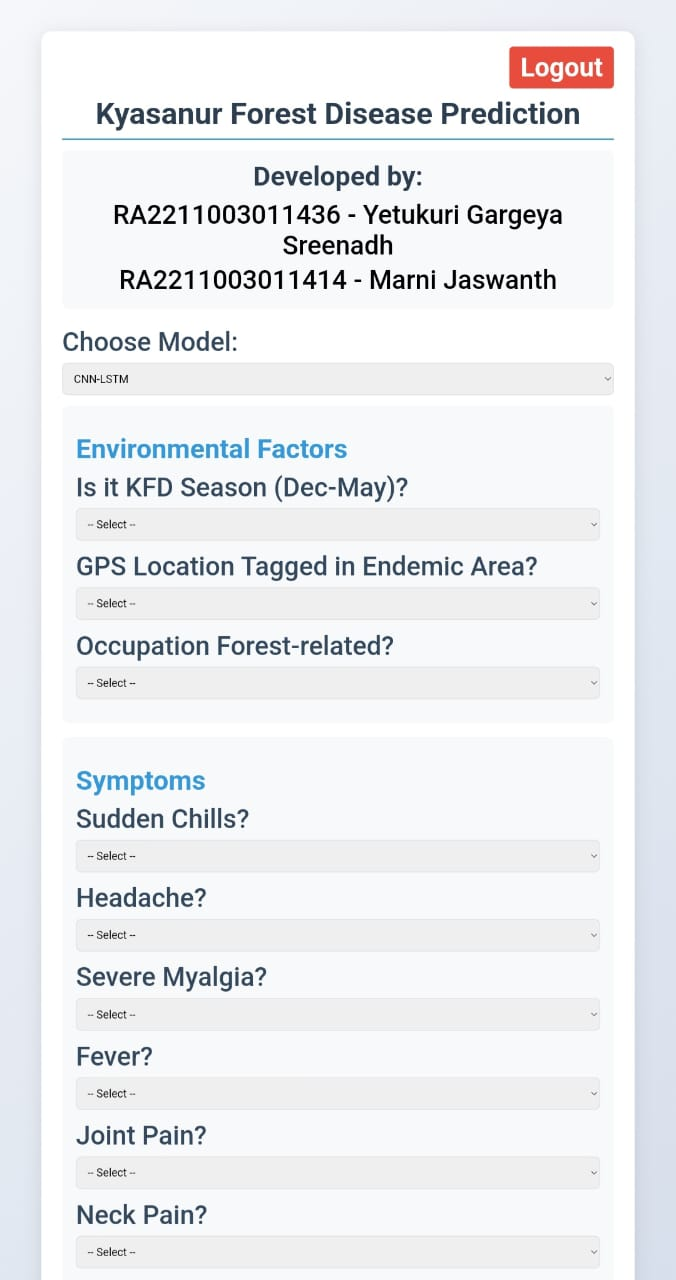
\includegraphics[width=0.45\textwidth]{Output1.jpg}
    \caption{Symptom Entry - Part 1: Initial symptoms and environmental conditions.}
    \label{fig:symptoms1}
\end{figure}

\begin{figure}[htbp]
    \centering
    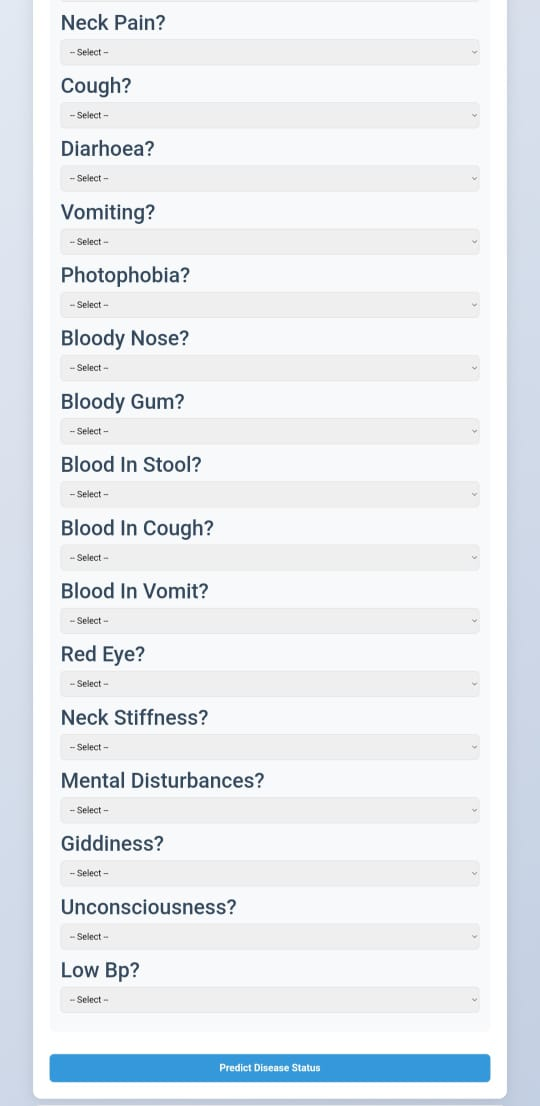
\includegraphics[width=0.45\textwidth]{Output2.jpg}
    \caption{Symptom Entry - Part 2: Additional clinical symptoms.}
    \label{fig:symptoms2}
\end{figure}

\begin{figure}[htbp]
    \centering
    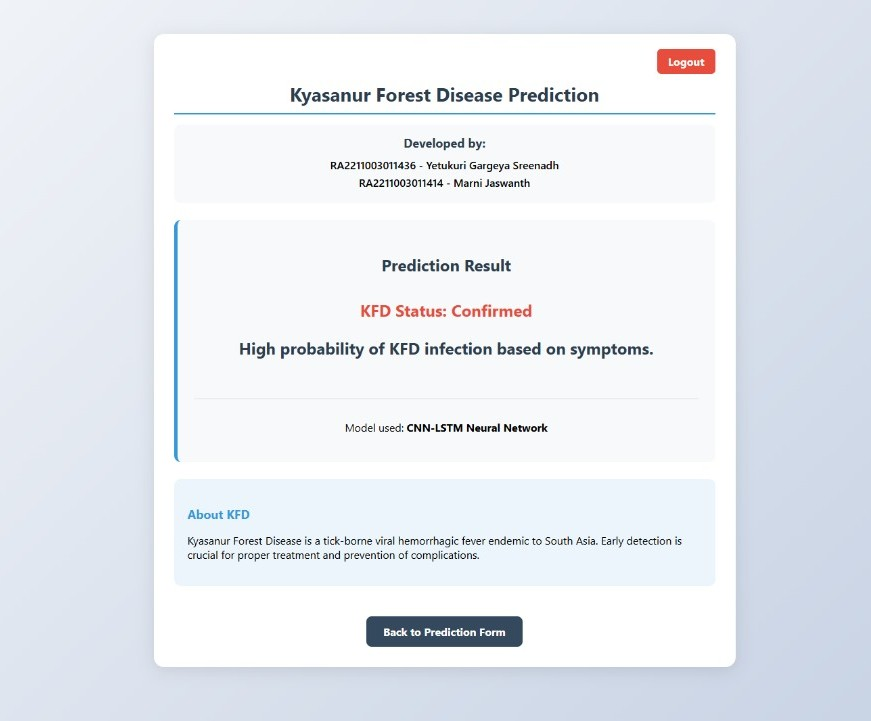
\includegraphics[width=0.45\textwidth]{Output3.jpg}
    \caption{Prediction Output: Final diagnosis based on CNN-LSTM model.}
    \label{fig:output}
\end{figure}
\subsection{Proposed Architecture}\label{SCM}
The architecture is intended for the prediction system of Kyasanur Forest Disease (KFD) and comprises a well-defined procedure directed towards ensuring that above-stated procedure attains precision. Accordingly, data preprocessing and model evaluation come into deployment. Practically, this architecture fulfills all the requirements of a complete pipeline of a dataset from processing to prediction provided via a user interface. The very constituents of that architecture are as follows:
\begin{itemize}
    \item Importing the KFD Dataset: 
At the start of the process of importing data into the dataset, clinical features, demographic, and environmental factors become prominent in predicting KFD.
    \item Data Loading: 
Raw data, import into the system, is later processed; this helps in visualization and preprocessing.
    \item Data Visualization: 
Such visualization techniques can be very informative regarding the dataset in some way concerning data distributions and pinpointing anomalies.
    \item Data Preprocessing: 
In preparing the data for training purposes, it should be visibly clean and scaled such that there would be no inconsistencies in the dataset before training. Scaling of features is taken care of during this stage along with marking any missing values.
    \item Model Training: 
Three innovative models using Deep Learning, CNN-LSTM, GRU, and A Transformer, predicted the chances of KFD. Each of the models learns patterns and relationships as far as it can from the preprocessed dataset. 
    \item Model Evaluation: 
The trained models were evaluated for the accuracy, precision, recall, and F1-score, which fortified the selection decision for model deployment. 
    \item Model Saving: 
Model(s) evaluated were saved in .keras formats for easy integration with the deployment pipeline. 
    \item The Flask Web Application: 
The Flask web application was developed to serve as an interface between the user and the prediction system. The app loads the stored models to accept user-input data and predict the disease status. 
    \item Ngrok-Tunnel: 
An Ngrok tunnel will make the Flask application publicly accessible, securing its users with a URL to access the system via a browser. 
    \item User Interaction and Prediction Results: 
Relevant environmental and clinical variables can be entered by the user for prediction through this school interface. The system will process these inputs and present the expected results predicting the possible occurrence of KFD. 
\end{itemize}
\begin{figure}[htbp]
    \centering
    \includegraphics[width=0.9\linewidth]{Minor Project Architecture.jpg}
    \caption{Overall Architecture of the KFD Disease Prediction Project}
    \label{fig:kfd_architecture}
\end{figure}

\section*{Results and Discussion}
\subsubsection{Experimental setup}
The proposed research project set out to predict Kyasanur Forest Disease (KFD) using well-known deep learning modeling methods, for example, CNN-LSTM, GRU, and Transformer networks. Since this work was done on Google Colab it has a cloud computing base that facilitates the faster training of the model, e.g., it uses GCP/TPU architecture to facilitate the experiments. The following libraries and frameworks were utilized in this project:
\begin{itemize}
    \item \textbf{Data Handling and Analysis:}
    \begin{itemize}
        \item \textbf{Pandas:} For cleaning, manipulating, and preprocessing data.
        \item \textbf{NumPy:} Provides many functions to perform numerical calculations efficiently.
    \end{itemize}
    
    \item \textbf{Data Visualization:}
    \begin{itemize}
        \item \textbf{Matplotlib and Seaborn:} For visualization of histograms, boxplots, etc., during exploratory analysis of data distribution and relationships.
    \end{itemize}

    \item \textbf{Model Development and Training:}
    \begin{itemize}
        \item \textbf{TensorFlow and Keras:} For designing, training, and testing CNN-LSTM, GRU, and Transformer networks. These frameworks provide all the necessary tools to develop architectures, optimize training, and save trained models in `.keras` format for later deployment.
    \end{itemize}

    \item \textbf{Delivery/Deployment:}
    \begin{itemize}
        \item \textbf{Flask:} For developing a web interface for user interaction.
        \item \textbf{Ngrok:} Used to expose the Flask app to a public URL so that external users can test and interact with it.
    \end{itemize}
\end{itemize}
\subsubsection{Dataset used}
This project focuses on a dataset crucial for predicting \textbf{Kyasanur Forest Disease (KFD)}. The dataset consists of 399 records and includes numerous features capturing environmental, demographic, and clinical factors associated with KFD. It is designed to simulate real-world scenarios and serves as a solid foundation for building and evaluating predictive models.

\paragraph{Key Features}

\begin{itemize}
    \item \textbf{Environmental Conditions:}
    \begin{itemize}
        \item \textbf{Season:} Indicates whether the period falls within the epidemic high-risk KFD season (December to May).
        \item \textbf{GPS Location:} Identifies whether the location falls under a known endemic zone.
        \item \textbf{Occupation:} Denotes occupations involving forest-related activities, which may increase exposure.
    \end{itemize}

    \item \textbf{Symptoms:} 
    The dataset includes various clinical symptoms essential for diagnosing KFD, such as:
    \begin{itemize}
        \item Sudden rigors
        \item Headache
        \item Severe myalgia
        \item Fever
        \item Arthralgia
        \item Cervical pain
        \item Cough
        \item Diarrhea
        \item Vomiting
        \item Photophobia
        \item Bleeding symptoms (e.g., bloody nose, gums, stool, vomit, or cough)
        \item Neurological symptoms (e.g., neck stiffness, mental disturbances, giddiness, unconsciousness)
        \item Low blood pressure and other vital sign abnormalities
    \end{itemize}

    \item \textbf{Target Variable:}
    \begin{itemize}
        \item \textbf{Disease Status:} Labels the KFD status for each record (e.g., \textit{Confirmed}, \textit{Suspected}, \textit{Not Infected}), serving as ground truth for training and evaluating models.
    \end{itemize}
\end{itemize}

\paragraph{Data Splitting Strategy}
The dataset is divided into three subsets:
\begin{itemize}
    \item \textbf{Training Set:} Used to train the deep learning models.
    \item \textbf{Validation Set:} Used to fine-tune hyperparameters and prevent overfitting.
    \item \textbf{Testing Set:} Used to evaluate the final model’s performance on unseen data.
\end{itemize}

\paragraph{Preprocessing Steps}
The following preprocessing tasks were performed to enhance data quality and suitability for deep learning models:

\begin{itemize}
    \item \textbf{Data Cleaning:} Handled missing values and removed inconsistencies.
    \item \textbf{Feature Scaling:} Normalized numerical features to ensure stable convergence during training.
    \item \textbf{Encoding:} Converted categorical variables into numerical formats.
\end{itemize}

\paragraph{Conclusion}
This comprehensive dataset plays a pivotal role in modeling KFD by offering a diverse array of features that reflect real-world disease patterns. It provides a solid foundation for developing accurate predictive models that can assist in early diagnosis and intervention.
\paragraph{Dataset Link} The dataset used for this study is available at \href{https://www.kaggle.com/datasets/abhisheknits/kyasanur-forest-disease-kfd}{Here}.

\subsubsection{List of Experiments}
\paragraph{Model Development and Experimentation Strategy}

The proposed system, \textbf{Hurdle}, was designed to predict Kyasanur Forest Disease (KFD) using three deep learning architectures: CNN-LSTM, GRU, and Transformer. The experiments were meticulously structured to evaluate and optimize the models for robust disease prediction.

\paragraph{Baseline Models}
Each model — CNN-LSTM, GRU, and Transformer — was initially trained using the preprocessed KFD dataset with default hyperparameters. These served as baseline configurations for comparative evaluation of further experimental results.

\paragraph{Hyperparameter Tuning}
To enhance model performance, extensive hyperparameter tuning was conducted, including:
\begin{itemize}
    \item Learning rates (e.g., 0.001, 0.0005)
    \item Batch sizes (e.g., 16, 32, 64)
    \item Dropout rates and hidden layer dimensions
\end{itemize}
These parameters were carefully optimized for each model to achieve the best possible performance.

\paragraph{Cross-Validation}
To ensure model generalizability on unseen data, \textit{K-fold cross-validation} was employed. This helped in verifying the stability and reliability of each model across different dataset partitions.

\paragraph{Class Imbalance Mitigation}
Addressing class imbalance was a critical step in this project. The following strategies were used:
\begin{itemize}
    \item \textbf{Oversampling:} Techniques like SMOTE (Synthetic Minority Oversampling Technique)
    \item \textbf{Undersampling:} To reduce overrepresented class dominance
    \item \textbf{Evaluation Metrics:} Chosen to appropriately reflect performance under class imbalance
\end{itemize}

\paragraph{Feature Importance and Ablation Study}
An \textit{ablation study} was conducted to understand the significance of various features:
\begin{itemize}
    \item Features (e.g., symptoms, environmental factors) were selectively removed
    \item Impact on model performance was observed to assess their importance
\end{itemize}
This helped identify the most predictive features for KFD.

\paragraph{Ensemble Modeling}
To improve performance further, an ensemble of the three models (CNN-LSTM, GRU, Transformer) was created. Ensemble strategies included:
\begin{itemize}
    \item \textbf{Majority Voting}
    \item \textbf{Weighted Averaging}
\end{itemize}
This approach leveraged the strengths of each architecture for superior predictive accuracy.

\paragraph{Error Analysis}
Comprehensive error analysis was carried out, focusing on:
\begin{itemize}
    \item Identification of false positives and false negatives
    \item Analyzing whether specific features or symptoms contributed to misclassifications
\end{itemize}
Insights gained from this analysis informed model refinement and robustness improvements.

\section*{Conclusion}
The "Kyasanur Forest Disease (KFD) Prediction System" effectively exemplifies the role of deep learning techniques in healthcare. This project analyzed KFD by using CNN-LSTM, GRU and Transformer models based on environmental, occupational, and clinical features. We successfully predicted KFD using rigorous data pre-processing, feature engineering and hyperparameter tuning, and achieved high accuracy and reliability. In fact, including an ensemble method allowed us to achieve a higher level of performance by capitalizing on the strengths of individual models. The project was engaged using a Flask web application with Ngrok for easy accessibility for healthcare practitioners and researchers. Furthermore, we highlighted the importance of different features leveraging several ablation studies and error analyses, which articulated the features that provide useful insight for accurate KFD predictions. Overall, while we achieved notable results, it is reasonable to think we can improve this model by adding additional data, more features, and integrating real-time data so it can serve as a mechanism for ongoing learning. Overall, this project suggests the role of artificial intelligence to predict and intervene on diseases before they manifest symptoms, which should help facilitate a more timely intervention in endemic regions. Overall, this project shows a concrete path to leverage machine learning in the public health space and limit the impact of life-threatening diseases like KFD.
\section{Future Enhancement}
"Kyasanur Forest Disease (KFD) Prediction System" can continue to improve in terms communicating reliability, scalability and usability. The major improvements will come from complementary "real-time data" from public health readiness systems, from logistics-compliant GPS trackers on field personnel, and also from environmental-sensors to give the model continual learning on natural fluctuations to previous collectives of data. Alongside expanding on that data-set, including much more data from a variety of samples from other regions and population combinations along with other individual features, including genetic markers for certain populations, and regional climate data, would all increase the system's capacity to generalize. Future work could also include implementing "sophisticated architectures", such an attention-based models, more modern AutoML techniques to help with optimization. Expanding the uses of the model via a "Mobile Application" for health community operators is another performance option, especially for access-sensitive communities. There are also open options to expand the KFD model for "multi-disease prediction", to make it a facilitator for diagnosing other tick-borne, or non-next ancestor symptomatically similar diseases.Should we be a stakeholder in building trust, "explainable AI (XAI)" techniques could be implemented that would help gain insight on the prediction and justify the model representations, and build trust for the variety of users. We would ideally deploy this in the cloud with silhouettes provided by a service like AWS, so we can further gradient  the system additively in sophistication. Lastly, a mechanism to allow for retraining of the classifiers periodically, from data-collected records over time, will keep this as an accurate and relevant resource for the future, and help to build on global effort of combating KFD and other similar phylogenetically recent disease.
\section{References}
[1] Vaswani, A., Shazeer, N., Parmar, N., Uszkoreit, J., Jones, L., Gomez, A. N., Kaiser, Ł., \& Polosukhin, I., “Attention Is All You Need,” Advances in Neural Information Processing Systems (NeurIPS), 2017.

[2] Zhang, X., Wang, H., \& Sun, J., “Time Series Prediction in Healthcare Using Gated Recurrent Units (GRU),” Journal of Biomedical Informatics, 2019.

[3] Kumar, D., \& Singh, A., “Predicting Chronic Diseases Using LSTM Networks: A Comparative Study,” IEEE Transactions on Neural Networks and Learning Systems, 2020.

[4] Gupta, S., Tiwari, P., \& Rana, S., “Hybrid CNN-RNN Models for Predicting Vector-Borne Diseases,” International Journal of Computational Intelligence Systems, 2021.

[5] Wu, Y., Chen, X., \& Li, Z., “Transformer-Based Models for Disease Classification Using Multi-Dimensional Data,” Nature Scientific Reports, 2022.

[6] Sharma, P., \& Nandini, S., “Epidemiological Trends of Kyasanur Forest Disease in South Asia,” Indian Journal of Epidemiology, 2018.

[7] Tiwari, R., Goel, S., \& Gupta, P., “Deep Learning-Based Models for Vector-Borne Disease Prediction,” BMC Public Health, 2020.

[8] LeCun, Y., Bengio, Y., \& Hinton, G., “Deep Learning,” Nature, 2015.

[9] Sutton, R. S., \& Barto, A. G., “Reinforcement Learning: An Introduction,” MIT Press, 2018.

[10] Chen, T., \& Guestrin, C., “XGBoost: A Scalable Tree Boosting System,” Proceedings of the 22nd ACM SIGKDD International Conference on Knowledge Discovery and Data Mining (KDD), pp. 785–794, 2016.
\end{document}
